%%%%%%%%%%%%%%%%%%%%%%%%%%%%%%%%%%%%%%%%%%%%%%%%%%%%%%%%%%%%%%%%%%
%%%%%%%% ICML 2014 EXAMPLE LATEX SUBMISSION FILE %%%%%%%%%%%%%%%%%
%%%%%%%%%%%%%%%%%%%%%%%%%%%%%%%%%%%%%%%%%%%%%%%%%%%%%%%%%%%%%%%%%%
\documentclass{article}
\usepackage{times}
\usepackage{graphicx} % more modern
\usepackage{subfigure} 
% For citations
\usepackage{natbib}
% For algorithms
\usepackage{algorithm}
\usepackage{algorithmic}

% Stuff that I added in (Daniel Seita) 
\usepackage{amsmath,amssymb,amsthm,verbatim}
\graphicspath{ {Images/} }
\newtheorem{thm}{Theorem}[section]
\newtheorem{conj}[thm]{Conjecture}
\newtheorem{cor}[thm]{Corollary}
\newtheorem{lem}[thm]{Lemma}
\newtheorem{prop}[thm]{Proposition}
\newtheorem{exa}[thm]{Example}
\newtheorem{defi}[thm]{Definition}
\newtheorem{exe}[thm]{Exercise}
\newtheorem{rek}[thm]{Remark}
\newtheorem{que}[thm]{Question}
\newtheorem{prob}[thm]{Problem}
\newtheorem{cla}[thm]{Claim}
% End of stuff I added in

% As of 2011, we use the hyperref package to produce hyperlinks in the resulting PDF.  If this breaks your system, please commend out the following
% usepackage line and replace \usepackage{icml2014} with \usepackage[nohyperref]{icml2014} above.
\usepackage{hyperref}

% Packages hyperref and algorithmic misbehave sometimes.  We can fix this with the following command.
\newcommand{\theHalgorithm}{\arabic{algorithm}}

% Employ the following version of the ``usepackage'' statement for submitting the draft version of the paper for review.  This will set the note in
% the first column to ``Under review.  Do not distribute.''
%\usepackage{icml2014} 
% Employ this version of the ``usepackage'' statement after the paper has been accepted, when creating the final version.  This will set the note in
% the first column to ``Proceedings of the...''
\usepackage[accepted]{icml2014}

% The \icmltitle you define below is probably too long as a header.  Therefore, a short form for the running title is supplied here:
\icmltitlerunning{The Distributed Retired Traveling Salesman Problem}

\begin{document} 

\twocolumn[
\icmltitle{The Distributed Retired Traveling Salesman Problem}

% It is OKAY to include author information, even for blind submissions: the style file will automatically remove it for you unless you've provided the
% [accepted] option to the icml2014 package.
\icmlauthor{Daniel Seita}{dts1@williams.edu}
\icmlauthor{Ziang Zhang}{zz2@williams.edu}
\icmladdress{Department of Computer Science, Williams College, Williamstown, MA 01267 USA}

% You may provide any keywords that you find helpful for describing your paper; these are used to populate the "keywords" metadata in the PDF but will
% not be shown in the document
\icmlkeywords{distributed systems}

\vskip 0.3in
]

\begin{abstract} 
The use of major online travel agencies has made scheduling long-term travel much easier by allowing users to easily identify a set of flights in just
a few clicks. Current travel agencies allow users to plan out long-term trips involving flights to more than two cities, but they require specific
arrival and departure dates for each city and a city ordering. We present a system that does not burden the user with these decisions. Specifically,
our code takes in two required inputs: a list of cities the user wishes to travel to, and a date range over which they are willing to travel, and
outputs the cheapest set of flights within that range that form a valid route. It essentially solves a harder version of the Traveling Salesman
Problem since costs are not constant between two cities. Under several weak assumptions, and assuming that the number of cities and days is
sufficiently limited, then our algorithm should successfully find the cheapest cost flight in a reasonable amount of time. We present the theoretical
and systematic components of the project and discuss empirical results.
\end{abstract} 

\section{Introduction and Motivation}\label{sec:intro}

The use of major online travel agencies, such as Travelocity\footnote{\url{www.travelocity.com}} and Kayak\footnote{\url{www.kayak.com}}, has made
scheduling long-term travel much easier by allowing users to easily select a set of flights to purchase tickets from. People use a combination of
factors to help them make their decision, such as the total price of the flights and the days they wish to land and depart from a city. Current travel
agencies allow users to plan out trips involving airlines to multiple destinations (see Figure~\ref{fig:travelocity} for an example using
Travelocity), but they require (1) specific dates for each city and (2) an ordering.

This limitation can make searching for flight routes time-consuming for users who are not restricted to arriving at cities on particular dates. For
instance, suppose one resides in New York City (NYC) and wants to schedule a summer trip to Paris, London, and Tokyo from June 1 to June 20, and it
does not matter to him how long he stays in a city. Suppose that it also does not matter the ordering that he arrives at the cities. Thus, the factors
that matter\footnote{For brevity, we list a high-level overview of the problem without getting into too many technical details;
Section~\ref{sec:limitations} describes additional assumptions we impose on the problem to make it practical.} are:

\begin{itemize}
    \item The full flight route occurs within the date range (in this case, between June 1 and June 20).
    \item The flight route must arrive and leave at least once for NYC, Paris, London, and Tokyo.
    \item The flight route is valid and logically consistent. For instance, if the first flight takes him from NYC to Tokyo, the second flight in the
    route should not depart from a place other than Tokyo.
\end{itemize}

There are a vast pool of valid flight routes. It is reasonable to assume that out of all these, one would want the \emph{cheapest} route.
Unfortunately, finding the cheapest route possible is challenging using current agencies, because they require knowing the arrival and departure dates
for each city. The reason for this is simple: the problem of finding this flight route is a hard problem to solve.

In fact, this problem is very similar to the well-known Traveling Salesman Problem~\cite{Applegate:2007:TSP:1374811}, which asks if there exists a
cycle in a graph that touches each node exactly once (i.e., a Hamiltonian Path). Each edge has a cost associated with it, and the decision version of
the problem, which asks if there exists a valid Hamiltonian path with cost bounded by $B$, is NP-complete~\cite{Kar72}. In our case, we do not force
the user to visit each city exactly once because the cheapest flight through a sequence of cities \emph{may require} visiting a city more than once.

What makes our problem (likely) much harder than the Traveling Salesman Problem is that the cost of an edge between two nodes in our graph (i.e., two
cities) is not constant, because flight prices frequently change. We coin our problem the ``Distributed Retired Traveling Salesman Problem.'' The
``Retired'' portion comes from how we assume that whoever is planning this trip is retired, because otherwise, how would he or she have the time and
money? The ``Distributed'' part is because we incorporate concepts from the design and practice of distributed systems to build software that can
tackle this problem. We discuss the mathematical and systems portions of our solution in Sections~\ref{sec:math} and~\ref{sec:systems}, respectively.

\begin{figure}[t]
\vskip 0.2in
\begin{center}
\centerline{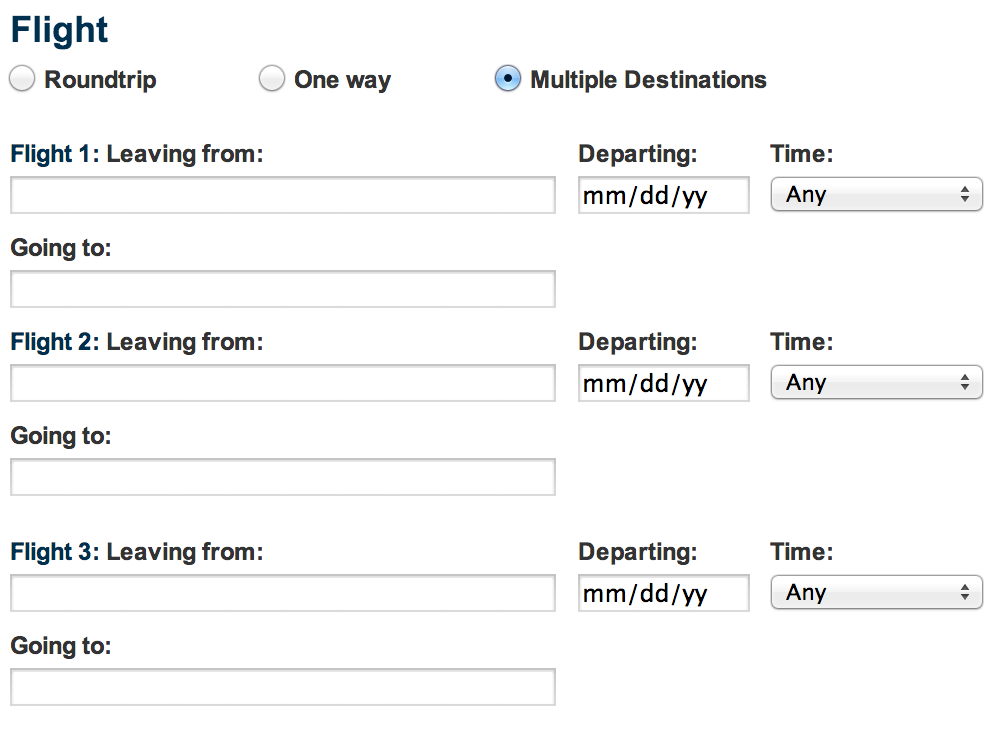
\includegraphics[width=\columnwidth]{travelocity}}
\caption{Travelocity lets users select multiple destinations.}
\label{fig:travelocity}
\end{center}
\vskip -0.2in
\end{figure}

\section{Related Work}\label{sec:related_work}

The Traveling Salesman Problem (TSP) is one of the oldest and most well-known problems in combinatorial optimization. While no exact, polynomial time
solution for the decision problem is known, there is a $3/2$-approximation algorithm due to Christofides~\cite{Chr76}. That algorithm was long the
standard approximation algorithm until a stunning recent result in~\cite{conf/focs/GharanSS11}, which has thus spurred a cascade of additional
research relating to the TSP (e.g.,~\cite{Moemke:2011:AGT:2082752.2082898}).

In contrast to the attention devoted to TSP, there appears to be very little research focusing on the special case of our problem, which introduces
additional challenges. These can be mathematically-oriented, such as how to manage the variable costs, or systems-oriented, such as how to even obtain
the actual flight costs. We have found nothing in the literature that particularly fits our problem.

\section{Mathematical Component}\label{sec:math}

The mathematical portion of our work uses a technique known as \emph{binary integer linear programming}, which falls under the broader category of
optimization techniques. The goal in optimization is straightforward: given a set of variables and a set of constraints, the goal is to find the best,
feasible solution according to some criteria, such as cost (in which case, ``best'' means ``minimal'').

\subsection{Linear and Integer Programming}

One of the most commonly-used optimization techniques is linear programming, introduced by Dantzig in~\cite{GVK180926950}.

\begin{defi}\label{defi:linear_programming}
A \emph{linear programming problem} consists of three components: 
\begin{enumerate}
    \item a finite collection of linear inequalities or equations in a finite number of unknowns, $x_1, \ldots, x_n$;
    \item sign constraints $x_i \ge 0$ on some (possibly empty) subset of the unknowns;
    \item a linear function to be minimized or maximized.
\end{enumerate}
An assignment to the variables $x_1, \ldots, x_n$ satisfying the first two conditions is a \emph{feasible} solution. If it also satisfies the third,
then it is an \emph{optimal} solution~\cite{opac-b1105716}.
\end{defi}

Linear programming has tremendous applications, and a full list of them would be impossible to create. Some problems well-suited to linear programming
include investment management, scheduling problems, and the diet problem. (The last problem concerns the rather interesting question of what is the
minimum cost of a nutritionally adequate diet.) The reason for linear programming's great versatility is the ease at which constraints can be added to
a model.

More specific cases of linear programming are integer and binary linear programming. (Sometimes we drop the ``linear'' part for brevity.)

\begin{defi}\label{defi:integer_programming}
An \emph{integer programming problem} is a linear programming problem with the added restriction that all variables (i.e., unknowns) $x_1, \ldots,
x_n$ are integers.
\end{defi}

\begin{defi}\label{defi:binary_programming}
A \emph{binary integer programming problem} is an integer programming problem with the added restriction that all variables $x_1, \ldots,
x_n$ are such that $x_i \in \{0,1\}$.
\end{defi}

We see that our problem is particularly suited to binary integer programming, because all the possible flights we could take can be viewed as a set of
binary random variables, each of which has value 1 if we decide to take that flight, and 0 otherwise. We now formulate this problem in more detail.

\subsection{An Integer Programming Formulation}

We define our problem formulation as follows.

\begin{itemize}
    \item We have $n$ cities to reach; we index cities by $i$ or $j$ (where $i, j \in \{1, 2, \ldots, n\}$).
    \item We have $t$ (consecutive) days when we can travel: $t \in \{1, 2, \ldots, m\}$. Let
    \item The minimum cost for traveling from city $i$ to $j$ on day $t$ is $c_{ijt}$. To start out this project, we assume that all flights span one
day and are not overnight, for simplicity. As soon as possible, we will expand this to include potential hub stops, overnight flights, etc.
\end{itemize}

This allows us to define the following binary variables:

\[
x_{ijt} = \begin{cases}
1 &\mbox{if we go from cities } i \mbox{ to } j \mbox{ on day } t, \\ 
0 & \mbox{otherwise}.
\end{cases}
\]

The goal is to solve this problem:

\begin{equation}
\mbox{Minimize } \sum_{t=1}^{m} \sum_{i=1}^{n} \sum_{j=1}^{n} c_{ijt}x_{ijt},
\end{equation}

\textbf{subject to} the following constraints:

\begin{align}
\sum_{i=1}^{n} \sum_{j=1}^{n} x_{ijt} &\le 1 \mbox{ for all } t \in \{1, 2, \ldots, m\}, \\ 
\sum_{t=1}^{m} \sum_{i=1}^{n} x_{ijt} &\ge 1 \mbox{ for all } j \in \{1, 2, \ldots, n\}, \\
\sum_{t=1}^{m} \sum_{j=1}^{n} x_{ijt} &\ge 1 \mbox{ for all } i \in \{1, 2, \ldots, n\}.
\end{align}

The first constraint ensures that we have at most one flight per day. The second constraint ensures we enter each city at least once. The third
constraint ensures we leave each city at least once. Sadly, this is \textbf{not} enough to solve our problem! The issue here is with potential cycles.
Figure~\ref{fig:bad_solution} shows how the integer programming solution could theoretically give us a solution consisting of disjoint cycles.

\begin{figure}[t]
\vskip 0.2in
\begin{center}
\centerline{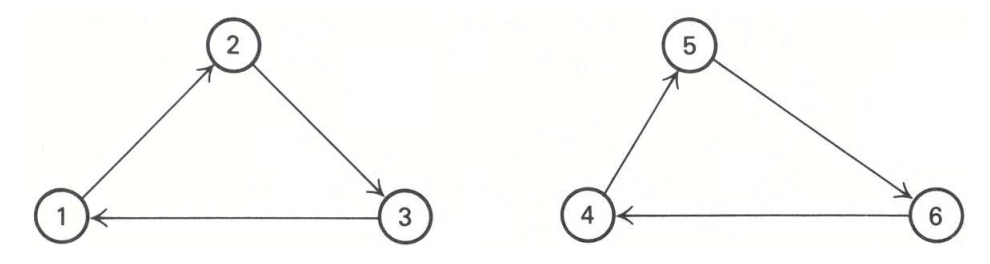
\includegraphics[width=\columnwidth]{bad_solution}}
\caption{This represents two sets of disjoint cycles.}
\label{fig:bad_solution}
\end{center}
\vskip -0.2in
\end{figure}

To counteract this issue, we will need to ensure we have additional variables. With the six-variable situation in Figure~\ref{fig:bad_solution}, for
instance, we will need constraints such as

\begin{equation}
\sum_{t=1}^{m} (x_{14t} + x_{15t} + x_{16t} + x_{24t} + x_{25t} + x_{26t} + x_{34t} + x_{35t} + x_{36t}) \ge 1.
\end{equation}

The previous constraint ensures that at least one leg of the tour connects cities 1, 2, and 3 with cities 4, 5, and 6. We need constraints like these
for every way we can split up the cities into groups. Of course, the need to implement these kind of constraints to prevent sub-tours is why integer
programming is so difficult. Fortunately, we will assume the user is going to keep the number of cities reasonably small.

here, we shoudl also add in prof miller's great example based on why int prog is so hard


\subsection{Implementation Details}

We will use the Matrix Airfare Search\footnote{\url{http://matrix.itasoftware.com/}} database to obtain information about our flights; the information
itself will be extracted with our own web crawler. We coin this ``The Retired Traveler Problem,'' primarily because if we assume the dates are set far
enough apart, it would interfere with a non-retired person's occupation. For details on the real problem, see sources such as.

How to best implement this is still an open question. There are algorithms for implementing integer programming. The question is whether we
can efficiently use our \emph{distributed systems}. There are a number of results based on parallelizing integer programming in the literature. We
will read through them and by the first checkpoint (see Section~\ref{sec:checkpoint1}) we will have made a decision. There are also some online
implementations, such as CPLEX Optimizer\footnote{\url{http://www-01.ibm.com/software/commerce/optimization/cplex-optimizer/index.html}}, but I think
it is in our best interests to implement this ourselves.

\section{Systems Component}\label{sec:systems}

\begin{figure}[t]
\vskip 0.2in
\begin{center}
\centerline{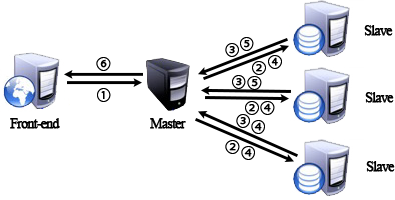
\includegraphics[width=\columnwidth]{servers}}
\caption{This represents our ideal machine setup.}
\label{fig:machines}
\end{center}
\vskip -0.2in
\end{figure}

We will have a front-end server, a master server, and a group of slave servers in the system, as shown in Figure~\ref{fig:machines}. We get all the
servers from the PlanetLab Platform (thanks to Jeannie).

\subsection{Front-end Server}
This server will serve as a front-end interface for the ignorant masses. It receives user input, forwards the request to the master server (shown in
the image as step \texttt{1}), listens to the master for the result (shown as step \texttt{6}), and displays the result when it is ready. More
specifically, the front-end server will have a simple website to interact with the user.

\subsection{Master Server}
The Master server is the brain of the system. It listens to the user request sent from the front-end server (step \texttt{1}). When a request comes
in, it first comes up with a list of flight prices on all possible dates and for all possible destinations in the problem that we need to get for the
computation, distributes the flight price queries among all the slaves (step \texttt{2}), gathers all the price data back from the slaves (step
\texttt{3}), and combines them. It then upload the combined data to a distributed file system to make the data available for parallel computing on all
the slaves. Then it starts the parallel computing for the cheapest route using a distributed zero-one linear programming algorithm on all slaves
(steps \texttt{4} and \texttt{5}). After the computation, it sends the results of the cheapest route back to the front-end server (step \texttt{6}).

\subsection{Slave Server}
We have a group of slave servers that listens to the command of the master server and does the distributed tasks of flight price querying (using the
web crawler we write) and parallel zero-one linear programming.

\section{Checkpoints}

\subsection{Checkpoint 5/2}\label{sec:checkpoint1}

By this date, we will have our machine/cluster and the web crawler working. We will finalize the mathematical portion of our work by choosing which
distributed algorithm to implement.

\subsection{Checkpoint 5/9}\label{sec:checkpoint2}

By this date, we will have implemented (1) the distributed systems requesting process\footnote{As stated earlier, this is when the master distributes
requests to slave machines to determine the cheapest flight for a certain date and city destinations.} and (2) the (possibly distributed) integer
programming problem.  In other words, the code will solve the problem for the two of us any reasonable input (it just lacks a front-end for the rest
of the ignorant masses). \\

{\bf UPDATE!!!} \\

We are now at the second checkpoint. Here is what we have accomplished:

\begin{itemize}
    \item We have implemented a web crawler
    \item We have implemented a web crawler server that can talk to the crawler to get the price
    \item We have implemented Balas' Additive Algorithm~\cite{doi:10.1287/opre.13.4.517} for efficiently solving binary integer programming problems.
    \item We have gotten the basic setup for our writeup (i.e., this PDF document) ... it just needs to be heavily revised.
\end{itemize}

We have sent all of our code to Jeannie by email.

I (Daniel Seita) have to admit that we're a bit behind where we want, because we haven't been able to actually combine our crawler's results with the
input to the integer programming problem, but we're going to do nothing but 339 work over the weekend. We're also thinking of expanding the work to
include other integer programming formulations (this is going to be an additional part of our mathematical side of this project).

\subsection{Presentation and Final Product}

By this date, we will have implemented a fancy front-end website where users can query a flight schedule. We will also be prepared to give a talk by
the May 13 ({\bf UPDATE: May 11}) date. Then we will work on fixing up this paper and doing some more programming.

\section{Limtiations}\label{sec:limitations}

{\bf TODO}

\section{Conclusions and Future Work}\label{sec:conclusions}

{\bf TODO}

\section*{Acknowledgments}
 
We thank Professor Jeannie Albrecht for teaching the course that inspired this project. We are also indebted to Professor Steven Miller for
introducing us to the world of operations research.

\bibliography{Daniel_Lucky_Report}
\bibliographystyle{icml2014}


% Jeannie doesn't need to read this if she doesn't want to...
\onecolumn

\appendix
\section{Balas' Additive Algorithm}

{\bf TODO}



\end{document} 

% Look at that! Andrea is here! ~Daniel Seita (05/08/2014)

% This document was modified from the file originally made available by
% Pat Langley and Andrea Danyluk for ICML-2K. This version was
% created by Lise Getoor and Tobias Scheffer, it was slightly modified  
% from the 2010 version by Thorsten Joachims & Johannes Fuernkranz, 
% slightly modified from the 2009 version by Kiri Wagstaff and 
% Sam Roweis's 2008 version, which is slightly modified from 
% Prasad Tadepalli's 2007 version which is a lightly 
% changed version of the previous year's version by Andrew Moore, 
% which was in turn edited from those of Kristian Kersting and 
% Codrina Lauth. Alex Smola contributed to the algorithmic style files.  
